%%%%%%%%%%%%%%%%%%%%%%%%%%%%%%%%%%%%%%%%%%%%%%%%%%%%%%%%%%%%%%%%%%%%%%%%%%%%%%%%
%2345678901234567890123456789012345678901234567890123456789012345678901234567890
%        1         2         3         4         5         6         7         8

\documentclass[letterpaper, 10 pt, conference]{ieeeconf}  % Comment this line out
                                                          % if you need a4paper
%\documentclass[a4paper, 10pt, conference]{ieeeconf}      % Use this line for a4
                                                          % paper

\IEEEoverridecommandlockouts                              % This command is only
                                                          % needed if you want to
                                                          % use the \thanks command
\overrideIEEEmargins
% See the \addtolength command later in the file to balance the column lengths
% on the last page of the document



% The following packages can be found on http:\\www.ctan.org
%\usepackage{graphics} % for pdf, bitmapped graphics files
%\usepackage{epsfig} % for postscript graphics files
%\usepackage{mathptmx} % assumes new font selection scheme installed
%\usepackage{times} % assumes new font selection scheme installed
\usepackage{amsmath} % assumes amsmath package installed
\usepackage{amssymb}  % assumes amsmath package installed
\usepackage{boldline}
\usepackage{array,multirow}
\usepackage{hyperref}
\usepackage{color}
\usepackage{graphicx}
\graphicspath{ {images/} }
\definecolor{light-gray}{gray}{0.95}
\newcommand{\code}[1]{\colorbox{light-gray}{\texttt{#1}}}
\DeclareMathOperator*{\argmax}{arg\,max}
\DeclareMathOperator*{\maxU}{max}
\usepackage{makecell}
\usepackage{bbm}
\usepackage[table,xcdraw]{xcolor}
\usepackage[flushleft]{threeparttable}
\usepackage[utf8]{inputenc}



\title{\LARGE \bf
Intuitive Features for Identifying Questions of Semantic Coincidence
}

\author{ \parbox{3 in}{\centering Tamir Bennatan
         {\tt\small tamir.bennatan@mail.mcgill.ca}}
         \hspace*{ 0.5 in}
         \parbox{3 in}{ \centering Pradeep Misra**
         {\tt\small pmisra@cs.wright.edu}}
}


\begin{document}



\maketitle
\thispagestyle{empty}
\pagestyle{empty}


%%%%%%%%%%%%%%%%%%%%%%%%%%%%%%%%%%%%%%%%%%%%%%%%%%%%%%%%%%%%%%%%%%%%%%%%%%%%%%%%
\begin{abstract}

This is a bunch of filler. It is here so that I don't screw myself over while formatting.This is a bunch of filler. It is here so that I don't screw myself over while formatting.This is a bunch of filler. It is here so that I don't screw myself over while formatting.This is a bunch of filler. It is here so that I don't screw myself over while formatting.This is a bunch of filler. It is here so that I don't screw myself over while formatting.This is a bunch of filler. It is here so that I don't screw myself over while formatting.This is a bunch of filler. It is here so that I don't screw myself over while formatting.This is a bunch of filler. It is here so that I don't screw myself over while formatting.This is a bunch of filler. It is here so that I don't screw myself over while formatting.This is a bunch of filler. It is here so that I don't screw myself over while formatting.This is a bunch of filler. It is here so that I don't screw myself over while formatting.This is a bunch of filler. It is here so that I don't screw myself over while formatting.This is a bunch of filler. It is here so that I don't screw myself over while formatting.This is a bunch of filler. It is here so that I don't screw myself over while formatting.

\end{abstract}


%%%%%%%%%%%%%%%%%%%%%%%%%%%%%%%%%%%%%%%%%%%%%%%%%%%%%%%%%%%%%%%%%%%%%%%%%%%%%%%%
\section{INTRODUCTION}

In January of 2017, Quora - a popular question and answer website - released a dataset consisting of pairs of questions from their site, and labels indicating if the questions have the same intent. Shortly thereafter, they used this dataset to start a Kaggle\footnotemark competition, offering \$25,000 to the competitors who build the best models for predicting if two questions are duplicates - meaning that they ask the same thing.

\footnotetext{Kaggle.com is a website which hosts data science and machine learning competitions.} 

The ability to identify duplicate questions is important for question-answer sites like Quora; duplicate questions make it harder to find the best answer for a particular question, and limit the outreach of each individual answer contributed to the site.

Identifying duplicate questions is a special case of the more general problem of identifying semantic coincidence between short texts. This problem arises in many Natural Language Processing (NLP) tasks, including information retrieval (Jurafsky \& Martin; 2009), automatic summarization (Lin \& Hovy; 2003) and text classification (Li \& Roth; 2002). 

In this paper, we describe three feature sets designed to capture  the semantic relationship between questions. We then evaluate the relative importance of these features for detecting duplicate questions. Each of these feature sets are inspired by different intuitions about what characterizes semantic similarity, and are engineered using techniques used in ranging NLP tasks.

The first feature set is based on Term Frequency-Inverse Document Frequency (Tf-Idf) scores. Tf-Idf scores have been shown to be an effective way to model the relative importance of words within a document (Rajaraman \& Ullman; 2011). As such, we propose a set of features which measure the similarity of two questions based on the similarity of the important words in each question.

The second feature set distinguishes between questions based a semantic categorization of its expected answer. Using a dataset of 6000 factoid questions, annotated with a categorization of their answers (Lin \& Roth; 2002), we fit a series of deep neural network models that predict the answer type of a question. We then used these models to predict the answer types of the questions in the Quora dataset, and used these predictions as features in our models.

The final feature set are a series of knowledge-based semantic similarity scores between paird questions. The similarity of two questions is calculated by composing the semantic similarities of the words in each question (Mihalcea et al; 2006), which can be computed in relation to a semantic network, such as WordNet (Miller; 1995). We also extend this framework by incorporating neural word embeddings to measure word-to-word similarity.

We first trained a classifier on a baseline set of syntactic and neural features. We then augmented this baseline with different subsets of the features mentioned above, and re-trained our classifiers with these new features. In this paper, we discuss the usefulness of our proposed feature sets in the duplicate question detection task.


\section{RELATED WORK}

To achieve high accuracy, many competitors in the Kaggle competition incorporated hundreds of features and stacked many classifiers when making predictions. Most successful competitors incorporated Long Short Term Memory Recurrent Neural Networks (LSTM) in their submissions. Two LSTM variants proved especially useful: Siamese LSTMs and LSTMs with neural attention.

Siamese LSTMs are composed of two or more LSTM layers which have tied weights. When trained on paired examples, Siamese LSTMs are though to construct sophisticated representations of semantic relationships between input texts, which makes them  effective in semantic similarity and entailment tasks (Mueller et al; 2016). This property is applicable to detecting question deduplication, since at its core the duplicate question detection task is one one of detecting semantic coincidence between pairs of input sentences.

Neural attention, when coupled with LSTMs, is a mechanism which allows a LSTM to pay selective attention to the outputs of intermediate LSTM units. This technique often improves the performance of LSTMs in  Natural Language Inference tasks (Rocktäschel et al.; 2016), and has proven effective for the Kaggle competition hosted by the Quora.

Our work differs from that of the top Kaggle competitors in that our main objective was not to maximize the performance of our models, but rather to craft novel linguistic features and evaluate their predictiveness. Thus, we did not focus on building sophisticated deep learning models, for it is typically difficult to determine the relative importance of different text features to a deep learning neural network. Instead, we focused on using tree-based models to measure the marginal increase in performance of our models when trained on each of our proposed feature sets.


\section{QUORA DATA SET}

The dataset released by Quora consists of 404290 pairs of questions posted to the site. 36.9\% of pairs are labeled as duplicates. There are no missing values [Table 1].  

\begin{table}[]
\centering
\caption{Sample of Quora Dataset}
\label{my-label}
\begin{tabular}{|p{29mm}|p{29mm}|p{15mm}|}
\hline
QUESTION 1                           & QUESITON 2 & DUPLICATE? \\ \hlineB{3}
How can I be a good geologist?                            & What should I do to be a great geologist? & 1 \\ \hline
What is a web application? & What is a web application framework?  & 0 \\ \hline
How can I access Torbox in India?                         & How can I access Google.com in India?     & 0 \\ \hline
\end{tabular}
\end{table}

Paired questions tend to be similar in that they are similarly worded, or in that they share words of low document frequency.

To guage the ambiguity of the task and the noisiness of the labels, we asked 8 native English speakers (not the authors) to each classify 40 randomly sampled question pairs as duplicates or not. Of the 320 human responses collected, 80.94\% coincided with the provided labels.


\section{METHOD}


\subsection{Baseline Features and Models} 

To determine if a new feature is useful, we built a baseline feature set and model, so that we could measure the increase in performance that results from incorporating each new feature set.

Our baseline feature set consists of standard syntactic and string distance features. We also noticed that many Kaggle competitors used neural word embeddings to construct “sentence vectors” for each question by averaging the embedding vectors of each word in a question. They then used various similarity functions to use the similarity between the sentence vectors of paired questions as features. We recreated these features using the fastText pre-trained word embeddings (Joulin et al.; 2016). Our initial features are summarized in Table 2.

\begin{table}[]
\centering
\caption{Baseline features}
\label{my-label}
\begin{tabular}{|p{15mm}|p{60mm}|}
\hline
Feature category                          & Feature \\ \hlineB{3}

Syntactic                        & Number of words in each question \\\cline{2-2}
features							   & Number of words the two questions have in common \\\hline

Character 				   & Number of character in each question \\\cline{2-2} 
 	features						   & Number of character in each question \\
\hline

Edit  		   & 	Partial string matches (with/without stopwords)			\\\cline{2-2}
distance 	& Token-wise string matches \\\cline{2-2}
variations \footnotemark		 				& Type-wise string matches \\\cline{2-2}
 								& Type-sorted string matches \\

\hline

Sentence embedding similarity \footnotemark	   & Vector similarities of sentence embeddings using Euclidean, Cosine, Cityblock, Bray-Curtis and Jaccard distances\\ 
				   	
\hline

\end{tabular}
\end{table}



\footnotetext[2]{Edit distance variations were computed using the python \emph{fuzzywuzzy} package. More information on these metrics can be found \href{http://chairnerd.seatgeek.com/fuzzywuzzy-fuzzy-string-matching-in-python/}{\color{blue} here.}}

\footnotetext[3]{Vector similarities were calculated using the python \emph{SciPy} package. More information on these metrics can be found \href{https://docs.scipy.org/doc/scipy/reference/spatial.distance.html}{\color{blue} here.}}


We then split the dataset into training and test splits, which we kept consistent in all further experiments. 
We trained Logistic Regression and Extremely Boosted Decision Trees (XGB) models on the training set using the features described in Table 2, and used 3-fold cross validation to tune hyperparameters. These are our baseline models. 

To test whether logistic regression and XGB models are adequate choices for this task, we also implemented an LSTM classifier, since many Kaggle competitors demonstrated that these models perform well on the Quora dataset. With the use of a development set, we compared serveral LSTM archetectures, and found that the Manhattan Siamese LSTM (MaLSTM) archetecutre (Mueller et al; 2016) performed best. 

The MaLSTM is a Siamese neural network which emits a prediction by taking the Manhattan similarity of of the vector representations of two inputs  where the Manhattan similarity of two vectors $v_1$ and $v_2$ is defined:
$$
    ManhattanSim(v_1, v_2) = \exp(-||{v_1 - v_2||_1})  \eqno{(1)}
$$
We used fastText word embeddings of the words in each question as inputs to the MaLSTM. More details on our chosen architecture can be found in Appendix 1. 

We found that the XGB model, when trained on the baseline featurees, had performance similar to that of the MaLSTM. Thus, we concluded that the XGB model has the capacity to adequately perform in the question duplicate detection task. 

\subsection{Tf-Idf Features}


Suppose that we were only allowed to compare one word from each question in a pair to determine if the questions are duplicates, but we had a choice of which words to compare. Which words should we choose? We would reasonably want to choose the most \emph{important} word from each question, or the words which are most particular to each question. 

For example, in the fabricated question pair:
\begin{enumerate}
\item \emph{Who is the president of the United States?} 
\item  \emph{What is the highest paying government position?}
\end{enumerate}
We would probably derive more insight into the similarity/dissimilarity of these questions by analyzing the words \emph{president} and \emph{government}, instead of more commonly occurring words, like \emph{who} and \emph{highest}.

We capture this intuition by creating a set of features that incorporate the Tf-Idf scores of each word. We used Scikit-Learn’s \code{TfidfTransformer} class  (Pedregosa et al.; 2011) to compute the Tf-Idf of a word $w$ in document $d$ using the formula:

$$
Tf\text{-}Idf(w, d) = Tf(w,d) * Idf(w) \eqno{(2)}
$$
Where $Tf(w,d)$ is the number of times word $w$ appers in document $d$ (term frequency), and $Idf(w)$ is defined:
$$
Idf(w) = \log{\frac{1 + n_d}{1 + df(w)}} + 1  \eqno{(3)}
$$
Where $n_d$ is the number of documents\footnote{\emph{Documents} and \emph{texts} are questions, in this context.} in the corpus, and $df(w)$ is the number of documents in the corpus that contain the word $w$. 

The Tf-Idf weight of a word in a document will be high if 1) the word appears many times in  that document, and 2) the word has low document frequency. It serves as a natural heuristic for modeling the relative importance of a word within a document. Tf-Idf weights are useful for many NLP tasks; in fact, variations of this scoring scheme are used to as term weights in nearly all vector space information retrieval models (Jurafsky \& Martin; 2012). 

Thus, we used Tf-Idf scores to craft four new features. The first two attempt to measure similarity of the “most important” word of each question in a pair. To do so, we find the word with the highest Tf-Idf weight in each question, take the fastText word embedding vectors for each of these words, and compute the distance between these vectors. We used cosine distance for one feature and Euclidean distance for the second. I.e:

$$
{Feature}_1 = ||Embed(w_1^*) - Embed(w_2^*)||_2 \eqno(4)
$$
$$
{Feature}_2 = \frac{\langle Embed(w_1^*), Embed(w_2^*) \rangle}{||Embed(w_1^*)||_2||Embed(w_2^*)||_2} \eqno(5)
$$
Where
$$
w_i^*= \argmax_{w_i \in d_i} \{ {Tf\text{-}Idf(w_i, d_i)}\} \quad \quad \quad  i \in \{1,2\}
$$

The third and fourth features measure the total Tf-Idf weight of the words two questions have in common, and the total weight of the words that they don’t: 

$$
{Feature}_3 = \sum_{w \in \{d_1 \cap d_2\}}{Tf\text{-}Idf(w, \{d_1 \cap d_2\})} \eqno(6)
$$
$$
{Feature}_4 = \sum_{w \in \{d_1 \bigtriangleup  d_2\}}\sum_{i = 1}^2{Tf\text{-}Idf(w, d_i)\mathbbm{1}(w \in d_i) } \eqno(7)
$$

\subsection{Question Classifcation Features}

IR-based question answering (QA) systems attempt to find short segments of text that adequately answer a user’s question by querying a database or searching the web (Jurafsky \& Martin; 2017). These systems tend to perform better if they first constrain the answer candidates using a semantic categorization of the expected answer of an input question (Li \& Roth; 2002).  

For example, when considering the question:
\begin{center}
\emph{Who is the president of the United States?}
\end{center}
A QA system should limit its search to words that correspand to humans, as opposed to considering all possible noun-phrases.

Using the Text Retrieval Conference (TREC) question dataset (Voorhees; 2002), Roth and Li (2005) developed a hierarchical taxonomy for classifying the answer type of a question; this taxonomy consists of 6 coarse categories, and 50 fine sub-categories. They then annotated the 6000 questions in the TREC dataset using this taxonomy. The coarse answer categories are LOCATION, DESCRIPTION, ENTITY, NUMERIC, HUMAN, and ABBREVIATION, and some examples of fine categories are NUMERIC:Date and NUMERIC:Money. The task of predicting the answer type of a question is broadly termed \emph{Question Classification}. 

We hypothesized that knowing the answer types of the questions in the Quora dataset would be useful for the question duplicate detection problem, since two questions are more likely to have duplicate intent if they share the same answer type. Our next feature set tests this hypothesis. 

We trained 5 LSTM models on the TREC dataset to predict the coarse categories of each question. These models had slightly different archetectures, but they all consisted of three layers:
\begin{enumerate}
\item Embedding layer using pretrained fastText 300-dimensional embeddings
\item LSTM layer of output dimension 50
\item Output layer (of varying types) of output dimension 6.
\end{enumerate}
The details of the different architectures are in Table 3. Note that we trained these LSTMs on the entire TREC dataset without the use of the development set,  so we make no statement about the performance of these models in the question classification problem. 


\begin{table}[]
\centering
\caption{Archetecture details of LSTM question classifiers }
\label{my-label}
\begin{tabular}{|p{10mm}|p{10mm}|p{10mm}|p{10mm}|p{14mm}|p{8mm}|}
\hline
Model  & Output Layer & Dropout  & Recurrent Dropout & Embeddings Trainable? & Input Length \\ \hline
LSTM 1 & Dense             & 20\%                   & -                 & NO                    & 10           \\
LSTM 2 & Dense             & -                      & 20\%              & NO                    & 10           \\
LSTM 3 & LSTM              & -                      & 20\%              & NO                    & 10           \\
LSTM 4 & LSTM              & 20\%                   & 20\%              & YES                   & 10           \\
LSTM 5 & LSTM              & -                      & 20\%              & NO                    & 6            \\ \hline
\end{tabular}
\end{table}

Using these models, we predicted the answer type of the questions in the the Quora dataset. Then, considering each LSTM model separately, we added these predictions to our baseline features, and measured the increase in our baseline XGB model using 3-fold cross validation. We also tried an ensemble approach, where the predicted class of each question is the class that was predicted the most frequently by the 5 LSTM models.

We found that the ensembled predictions, as well as a binary feature which indicates if these predictions coincide, increased the performance of our baseline XGB model the most (in terms of reduction of log-loss). Thus, these are the features in the second feature set which we propose: 
$$
Feature_5 = \text{\{Question 1 Answer Type Prediction\}}
$$
$$
Feature_6 = \text{\{Question 2 Answer Type Prediction\}}
$$
$$
Feature_7 = \mathbbm{1}(\text{Answer Type Predictions Agree?})\quad
$$
\subsection{Sentence Semantic Similarity Scores}

Our final feature set uses a framework for measuring the semantic similarity of short texts proposed by Mihalcea et al (2006). This framework models the similarity of two texts as a function of the similarities of their component words and the specificity of each word. Word-to-word similarities are measured with respect to a semantic knowledge base (e.g. WordNet.)

Given a word-to-word similarity metric, $Sim(w_1, w_2)$, and two texts\footnotemark[4] $T_1,$ $T_2$, the semantic similarity score of these two texts is computed by:
\begin{enumerate}
\item For each word $w \in T_1$, find the word $w^* \in T_2$ which maximizes $Sim(w, w^*)$.
\item Apply this same process to determine the words in $T_1$ that have the highest similarity to the words in $T_2$. 
\item Sum up the similarities (weighted by a measure of specificity, such as $Idf$ $(3)$), and normalize for the length of the sequences. 
\end{enumerate}
Note that words in one text are only compared to words in the other text \emph{of the same part of speech}, as many knowledge-based similarity measures cannot be applied across parts of speech (Mihalcea et al; 2006).

\begin{gather*} \tag{8}
SimText(T_1,T_2) = \\ \frac{1}{2}\Big( \frac{\sum_{w \in T_1}{\maxU_{w^* \in T_2}Sim(w,w^*)Idf(w)}}{\sum_{w \in T_1}Idf(w)} \\ + \frac{\sum_{w \in T_2}{\maxU_{w^* \in T_1}Sim(w,w^*)Idf(w)}}{\sum_{w \in T_2}Idf(w)} \Big)
\end{gather*}
This framework has the convenient properties of symmetry: $SimText(T_1, T_2)$ = $SimText(T_2, T_1)$, and that the range of the text similarity scores is the same as that of the word-to-word similarity measure  $Sim(w_1, w_2)$ used. 

We used the python NLTK package for part-of-speech tagging (Bird et al; 2009). We implemented this framework using three similarity metrics available via NLTK’s WordNet interface - path similarity, Leacock-Chodorow similarity (Leacock \& Chodorow; 1998) and Wu-Palmer similarity (Wu \& Palmer; 1994). 

We implemented one implication of this framework. First, we removed the dependency on $Idf$ scores in (4), and normalized by taking the average of the word-to-word similarities:

\begin{gather*} \tag{9}
SimText_{simplified}(T_1,T_2) = \\ \frac{1}{2}\Big( \frac{\sum_{w \in T_1}{\maxU_{w^* \in T_2}Sim(w,w^*)}}{|T_1|} \\ + \frac{\sum_{w \in T_2}{\maxU_{w^* \in T_1}Sim(w,w^*)}}{|T_2|} \Big)
\end{gather*}
We made this simplification to reduce the correlation between these similarity scores and the Tf-Idf features proposed in section 4.B - which also depend on Idf scores.

We also extended this model by using a word-to-word similarity scores based neural embeddings. Using pre-trained GloVe word embeddings (Pennington et al.; 2014) available through the SpaCy python library, we used the cosine similarity (5) of the embeddings of two words as the similarity function $Sim(w_1,w_2)$ in (8) and (9). 

Using 3-fold cross validation, we added different subsets of these text-to-text similarity scores to our baseline feature set, and studied resulting boost in our baseline XGB model performance. Since the text-to-text scores are highly correlated when using path similarity, Leacock-Chodorow similarity and Wu-Palmer similarity as $Sim(w_1, w_2)$, we only tested one of these scores at a time. 

We found that including two semantic similarity scores, calculated using the simplified scheme (9) and $Sim(w_1, w_2)$ as  Leacock-Chodorow distnace and embedding Cosine, resulted in the largest increase in performance in our baseline model. These two similarity scores define the inal feature set we propose. 

\begin{gather*} \tag{10}
Feature_{10} = \{SimText_{Simplified}(T_1, T_2) \\ \text{where } Sim(w_1, w_2) \equiv \text{Leacock-Chodorow Similarity}\}
\end{gather*}
\begin{gather*} \tag{11}
Feature_{11} = \{SimText_{Simplified}(T_1, T_2) \\ \text{where } Sim(w_1, w_2) \equiv \text{Cosine Distance (GloVe Embeddings)}\}
\end{gather*}


\section{RESULTS}

To measure the importance of each of these feature sets, we trained logistic regression and XGB models on all the features described above, using 3-fold cross validation to tune hyperparameters. We then removed different groups subsets of the Tf-Idf, question classification and semantic scoring feature sets, and re-tuned the models’ hyperparameters. We then used these models to predict the test-set labels. The prediction accuracy for the resulting XGB and Logistic Regression classifiers are summarized in table 4, as well as those of our baseline classifiers described in section 4.A. 

% Please add the following required packages to your document preamble:
% \usepackage[table,xcdraw]{xcolor}
% If you use beamer only pass "xcolor=table" option, i.e. \documentclass[xcolor=table]{beamer}
\begin{table*}[]
\centering
\caption{Test set accuracy scores, with different feature sets omitted}
\label{my-label}
\begin{threeparttable}
\begin{tabular}{|
>{\columncolor[HTML]{EFEFEF}}l |c|c|c|c|c|c|c|c|}
\hline
\multicolumn{9}{|c|}{\cellcolor[HTML]{ECF4FF}XGB  AND LOGISTIC REGRESSION, WITH FEATURE SETS OMITTED}                                                                                                                                                                \\ \hline
Feature sets ommited                                                            & $\emptyset$    & \{1\}                & \{2\}                & \{3\}                & \{1,2\}       & \{1,3\}                       & \{2,3\}                      & \{1,2,3\}     \\ \hline
XGB Test Set Accuracy                                                           & \textbf{.7925} & .7624 (.0301)        & .7861 (.0064)        & .7825 (.01)          & .7585 (.034)  & .7504 (.0421)                 & .7794 (.0131)                & .7456 (.0469) \\ \hline
\begin{tabular}[c]{@{}l@{}}Logistic Regression\\ Test Set Accuracy\end{tabular} & \textbf{.6962} & .6838 (.0124)        & .6951 (.0011)        & .6837 (.0125)        & .6836 (.0126) & .6743 (.0219)                 & .6827 (.0125)                & .6728 (.0234) \\ \hline
\multicolumn{9}{|c|}{\cellcolor[HTML]{ECF4FF}BASELINE MODELS}                                                                                                                                                                                                        \\ \hline
\multicolumn{1}{|c|}{\cellcolor[HTML]{EFEFEF}Manhattan LSTM}                    & .7588          & \multicolumn{3}{c|}{\cellcolor[HTML]{EFEFEF}Human (320 Responses)} & .8094         & \multicolumn{2}{c|}{\cellcolor[HTML]{EFEFEF}Random Guessing} & .5015         \\ \hline
\end{tabular}
\begin{tablenotes}
\item Here, \{1\} are the Tf-Idf features from 4.B, \{2\} are the question classification features from 4.C, and \{3\} are the sematantic similarity scores from 4.D.
\item Cells contain each model's prediction accuracy, as well as the difference between prediction accuracy and the best model's prediction accuracy. 
\end{tablenotes}
\end{threeparttable}
\end{table*}

\subsection{Headings, etc}

Text heads organize the topics on a relational, hierarchical basis. For example, the paper title is the primary text head because all subsequent material relates and elaborates on this one topic. If there are two or more sub-topics, the next level head (uppercase Roman numerals) should be used and, conversely, if there are not at least two sub-topics, then no subheads should be introduced. Styles named ÒHeading 1Ó, ÒHeading 2Ó, ÒHeading 3Ó, and ÒHeading 4Ó are prescribed.

\subsection{Figures and Tables}

Positioning Figures and Tables: Place figures and tables at the top and bottom of columns. Avoid placing them in the middle of columns. Large figures and tables may span across both columns. Figure captions should be below the figures; table heads should appear above the tables. Insert figures and tables after they are cited in the text. Use the abbreviation ÒFig. 1Ó, even at the beginning of a sentence.


Figure Labels: Use 8 point Times New Roman for Figure labels. Use words rather than symbols or abbreviations when writing Figure axis labels to avoid confusing the reader. As an example, write the quantity ÒMagnetizationÓ, or ÒMagnetization, MÓ, not just ÒMÓ. If including units in the label, present them within parentheses. Do not label axes only with units. In the example, write ÒMagnetization (A/m)Ó or ÒMagnetization {A[m(1)]}Ó, not just ÒA/mÓ. Do not label axes with a ratio of quantities and units. For example, write ÒTemperature (K)Ó, not ÒTemperature/K.Ó

\section{CONCLUSIONS}

A conclusion section is not required. Although a conclusion may review the main points of the paper, do not replicate the abstract as the conclusion. A conclusion might elaborate on the importance of the work or suggest applications and extensions. 

\addtolength{\textheight}{-12cm}   % This command serves to balance the column lengths
                                  % on the last page of the document manually. It shortens
                                  % the textheight of the last page by a suitable amount.
                                  % This command does not take effect until the next page
                                  % so it should come on the page before the last. Make
                                  % sure that you do not shorten the textheight too much.

%%%%%%%%%%%%%%%%%%%%%%%%%%%%%%%%%%%%%%%%%%%%%%%%%%%%%%%%%%%%%%%%%%%%%%%%%%%%%%%%



%%%%%%%%%%%%%%%%%%%%%%%%%%%%%%%%%%%%%%%%%%%%%%%%%%%%%%%%%%%%%%%%%%%%%%%%%%%%%%%%



%%%%%%%%%%%%%%%%%%%%%%%%%%%%%%%%%%%%%%%%%%%%%%%%%%%%%%%%%%%%%%%%%%%%%%%%%%%%%%%%
\section*{APPENDIX}

   \begin{figure}[thpb]
      \centering
      \framebox{\parbox{3in}{
      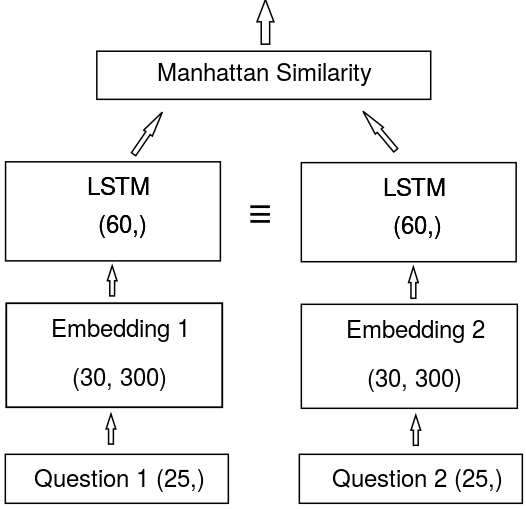
\includegraphics[scale=.2]{MaLSTM}
		\centering
      }}
      %\includegraphics[scale=1.0]{figurefile}
      \caption{Manhattan Siamese LSTM archetecture, annotated with output dimension at each layer. Weights of each LSTM layer are tied (Siamese).}
      \label{figurelabel}
   \end{figure}



\section*{STATEMENT OF CONTRIBUTION}

The preferred spelling of the word ÒacknowledgmentÓ in America is without an ÒeÓ after the ÒgÓ. Avoid the stilted expression, ÒOne of us (R. B. G.) thanks . . .Ó  Instead, try ÒR. B. G. thanksÓ. Put sponsor acknowledgments in the unnumbered footnote on the first page.



%%%%%%%%%%%%%%%%%%%%%%%%%%%%%%%%%%%%%%%%%%%%%%%%%%%%%%%%%%%%%%%%%%%%%%%%%%%%%%%%

References are important to the reader; therefore, each citation must be complete and correct. If at all possible, references should be commonly available publications.



\begin{thebibliography}{99}

\bibitem{c1} Daniel Jurafsky and James H. Martin. 2009. Speech and Language Processing (2nd Edition). Prentice-Hall, Inc., Upper Saddle River, NJ, USA.
\bibitem{c2} Daniel Jurafsky and James H. Martin. 2017 Speech and Language Processing. (3rd Edition Draft) 
\bibitem{c3} Lin, C., and Hovy, E. 2003. Automatic evaluation of summaries
using n-gram co-occurrence statistics. In Proceedings of Human
Language Technology Conference .
\bibitem{c4} Xin Li, Dan Roth, Learning Question Classifiers. COLING'02, Aug., 2002.
\bibitem{c5} Rajaraman, A.; Ullman, J.D. (2011). "Data Mining". Mining of Massive Datasets. pp. 1–17.
\bibitem{c6} Rada Mihalcea, Courtney Corley, and Carlo Strapparava. Corpus-based and knowledge-based measures of text semantic similarity. In AAAI’06, July 2006.
\bibitem{c7} George A. Miller (1995). WordNet: A Lexical Database for English. 
Communications of the ACM Vol. 38, No. 11: 39-41.
\bibitem{c8} Jonas Mueller and Aditya Thyagarajan. Siamese Recurrent Architectures for Learning Sentence Similarity. In AAAI, 2016
\bibitem{c9} Rocktäschel, Grefenstette, Hermann, Kočiský and Blunsom. Reasoning about Entailment with Neural Attention. in: International Conference on Learning Representations (ICLR). 2016
\bibitem{c10} A. Joulin, E. Grave, P. Bojanowski, T. Mikolov, Bag of Tricks for Efficient Text Classification
\bibitem{c11} Scikit-learn: Machine Learning in Python, Pedregosa et al., JMLR 12, pp. 2825-2830, 2011.
\bibitem{c12} Xin Li and Dan Roth, (2005). Learning question classifiers: The role of semantic information. Journal of Natural Language Engineering, 11(4).
\bibitem{Bird, Steven, Edward Loper and Ewan Klein (2009). Natural Language Processing with Python.  O'Reilly Media Inc.}
\bibitem{Wu, Z., and Palmer, M. 1994. Verb semantics and lexical selection. In Proceedings of the Annual Meeting of the Association for Computational Linguistics.}
\bibitem{Leacock, C., and Chodorow, M. 1998. Combining local context and WordNet sense similarity for word sense identification. In WordNet, An Electronic Lexical Database. The MIT Press.}
\end{thebibliography}




\end{document}
